\chapter{Desarrollo de IPFShare}\label{chap:4desarrollo}
Se ha denominado IPFShare al sistema de intercambio de archivos desarrollado en este proyecto.
\section{Requisitos y definición del sistema}
En esta sección se definen los requisitos funcionales y no funcionales que debe integrar el sistema propuesto.
\subsection{Requisitos funcionales}
\begin{itemize}[noitemsep,after=\vspace{-0.6\baselineskip}]
  \item Un usuario debe poder autenticarse en el sistema.
  \item Un usuario debe poder compartir archivos y directorios con uno o varios usuarios.
  \item Un usuario debe poder descargar archivos y directorios compartidos por otros usuarios del sistema.
  \item A la hora de compartir un archivo un usuario debe poder elegir con qué otros usuarios del sistema compartirlo.
  \item Un usuario debe tener posibilidad de hacer grupos de compartición.
  \item Cuando un usuario comparta recursos con otros usuarios, estos deben recibir una notificación.
  \item Un usuario debe poder interactuar las comparticiones que ha realizado.
  \item Un usuario debe poder interactuar las comparticiones que le han realizado.
\end{itemize}
\subsection{Requisitos no funcionales}
\begin{itemize}[noitemsep,after=\vspace{-0.4\baselineskip}]
  \item El sistema debe proporcionar una interfaz de usuario intuitiva y fácil de usar.
  \item El sistema debe implementar servicios de seguridad en torno a la autenticación.
  \item El sistema debe proporcionar medidas de seguridad para los archivos compartidos.
  \item El sistema debe proporcionar un servicio o mecanismos de identificación de usuario portable.
  \item Las transacciones y eventos del sistema deben ser relativamente instantáneos.
\end{itemize}
Hay que destacar que este sistema no propone la sincronización de archivos que normalmente se asocia con los sistemas de
almacenamiento en la nube. Incluir el desarrollo de esta funcionalidad en el sistema propuesto no es algo trivial.
La sincronización de datos en tiempo real es un tópico muy complejo y se sale
del alcance de este proyecto. Sin embargo, en la sección de \nameref{chap:7trabajosfuturos} dentro de las posibles
mejoras se propone una posible implementación de esta funcionalidad.
\section{Arquitectura y diseño}

Uno de los objetivos de este trabajo es comparar la viabilidad de IPFS como alternativa a los sistemas centralizados.
En esta sección se presenta una arquitectura simplificada para un sistema de intercambio de archivos centralizado habitual.
Después se contrastará con la alternativa descentralizada propuesta.

\subsection{Arquitectura de un sistema de intercambio de archivos centralizado habitual}

Como se puede observar en la figura \ref{fig:centralizedarch}, la arquitectura de un sistema de intercambio de archivos
requiere de varios puntos de acceso centralizados para funcionar\footnote{Este diseño se ha ideado tomando como referencia los siguientes recursos:
  \cite{chakrabortySystemDesignAnalysis2020} y
  \cite{systemdesignSystemDesignInterview2023}.}.En un caso real esta arquitectura podría ser más compleja, implementando sistemas de caching, entre otras muchas mejoras posibles. Para este ejemplo se ha simplificado para centrarse en los puntos clave.

Existe una clara separación conceptual de las distintos componentes, aunque pueden estar ubicados en
el mismo servidor físico, en varios, o incluso, cada servicio en varios servidores físicos. Esto depende de la escala
del sistema y de las necesidades de rendimiento y disponibilidad.

\begin{itemize}[noitemsep,after=\vspace{-0.4\baselineskip}]
  \item \textbf{Almacenamiento cloud:} el almacén donde se guardarán los chunks de ficheros proporcionados por el servicio
        de procesamiento de ficheros, Amazon S3 es un ejemplo de un servicio de estas característica.
        \item\textbf{Servicio de procesamiento de ficheros:} es el encargado atender y llevar a cabo las peticiones de usuario relacionadas con ficheros.
  \item \textbf{Servicio de autenticación:} gestiona la autenticación de los usuarios. Contiene los datos de los usuarios y sus credenciales.
  \item \textbf{Servicio de metadatos:} se encarga de enviar las notificaciones de los usuarios. Cuando un cliente
        comparte un fichero con otro, el cliente envía también una serie de metadatos sobre esta acción que acaba de realizar.
        Estos metadatos se pueden usar para gran variedad de propósitos. En este caso se usan para implementar un servicio de notificaciones basado en colas de mensajes.
\end{itemize}
\begin{sidewaysfigure}
  \centering
  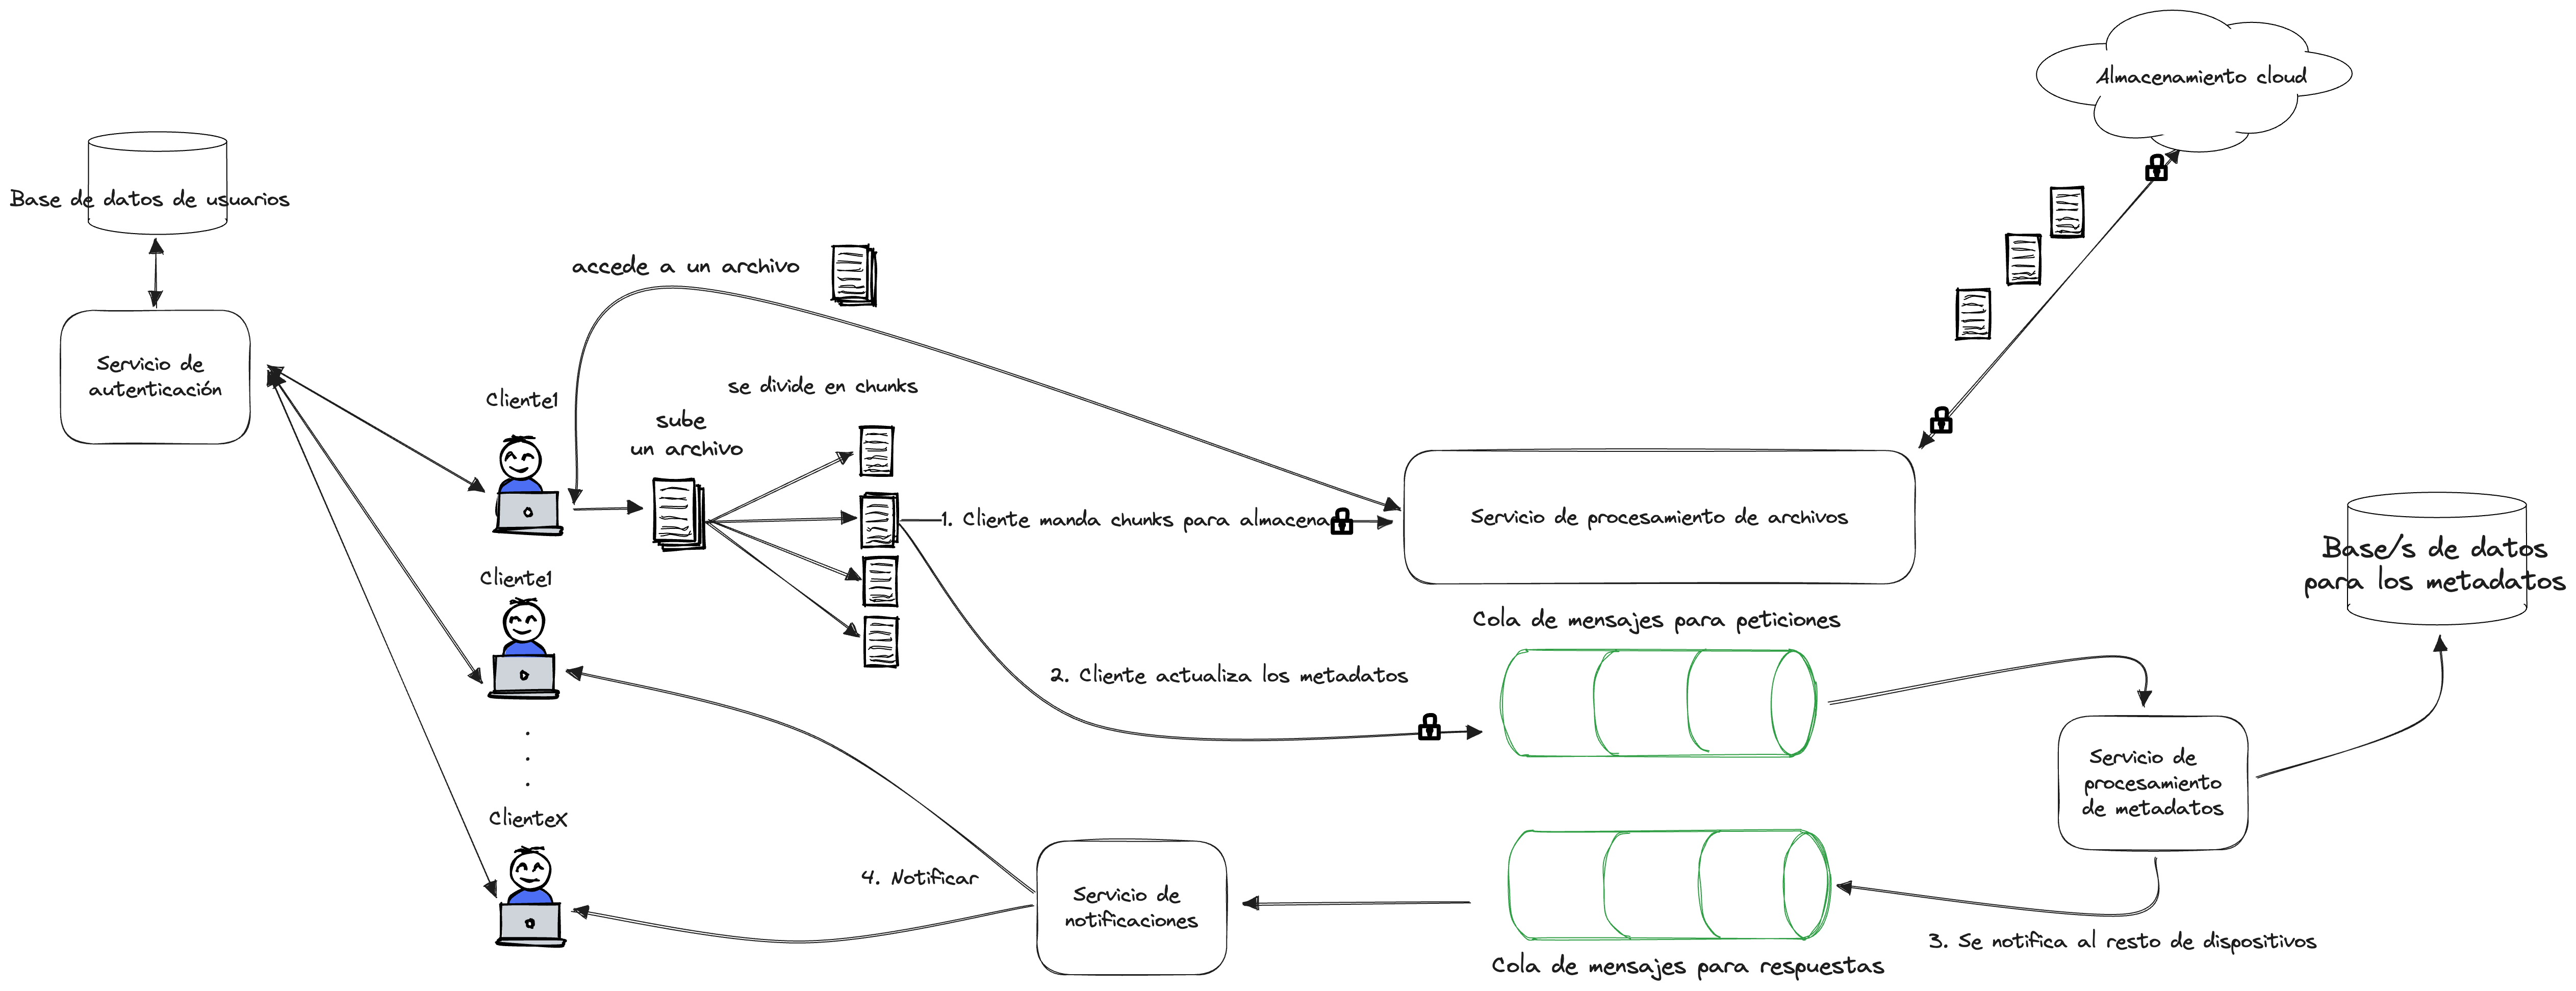
\includegraphics[width=\textwidth]{images/diagramacentral.png}
  \caption{Posible arquitectura de un servicio centralizado de archivos}
  \label{fig:centralizedarch}
\end{sidewaysfigure}

Cuando un cliente quiere compartir un fichero, este divide el archivo en trozos más pequeños llamados chunks\footnote{En un servicio de compartición de archivos, los archivos se subdividen en fragmentos o chunks para mejorar la eficiencia de la transferencia de datos, permitiendo la transmisión paralela y la reanudación de las transferencias interrumpidas, así como facilitar la distribución del almacenamiento y reducir la redundancia de datos.}.
Envía a través de una conexión segura (socket tpc sobre TLS por ejemplo) estos chunks que componen el archivo al servicio de procesamiento de ficheros.
Este servicio se encarga de guardar los chunks en el almacenamiento cloud y de mandar los metadatos a la cola de mensajes.
El servicio de metadatos procesa de forma asíncrona estos metadatos, extrayendo la información pertinente que identifique
a los usuarios y el recurso compartido. Después envía una notificación a los usuarios que corresponda.

Dado que el servicio de autenticación posee datos de los usuarios, cuando un usuario quiera enviar un archivo puede
pedir esta al servicio de autenticación, el incluso se podría combinar con el servicio de metadatos para brindar otras funcionalidades como ver los recursos que se le han compartido o los usuarios con los que se ha compartido.

Bajo este sistema los clientes deben saber de antemano dónde se ubican estos servicios para poder interactuar con
ellos. Estos servicios podrían ser provistos por entidades externas (lo cual es muy habitual en un sistema de este estilo), creando dependencias en
sistemas centralizados de terceros.
\subsection{Arquitectura de IPFShare: un sistema de intercambio de archivos descentralizado}
En comparación con la arquitectura anterior (figura \ref{fig:centralizedarch}), la arquitectura de IPFShare es
completamente descentralizada. No existe ningún servicio centralizado, cualquier servicio proporcionado por una entidad externa proviene de
de otros nodos IPFS, siendo el propio nodo cliente otro proveedor más de servicios. Esto hace el sistema completamente autocontenido e independiente de servicios fuera
de la red IPFS.

\begin{figure}[H]
  \centering
  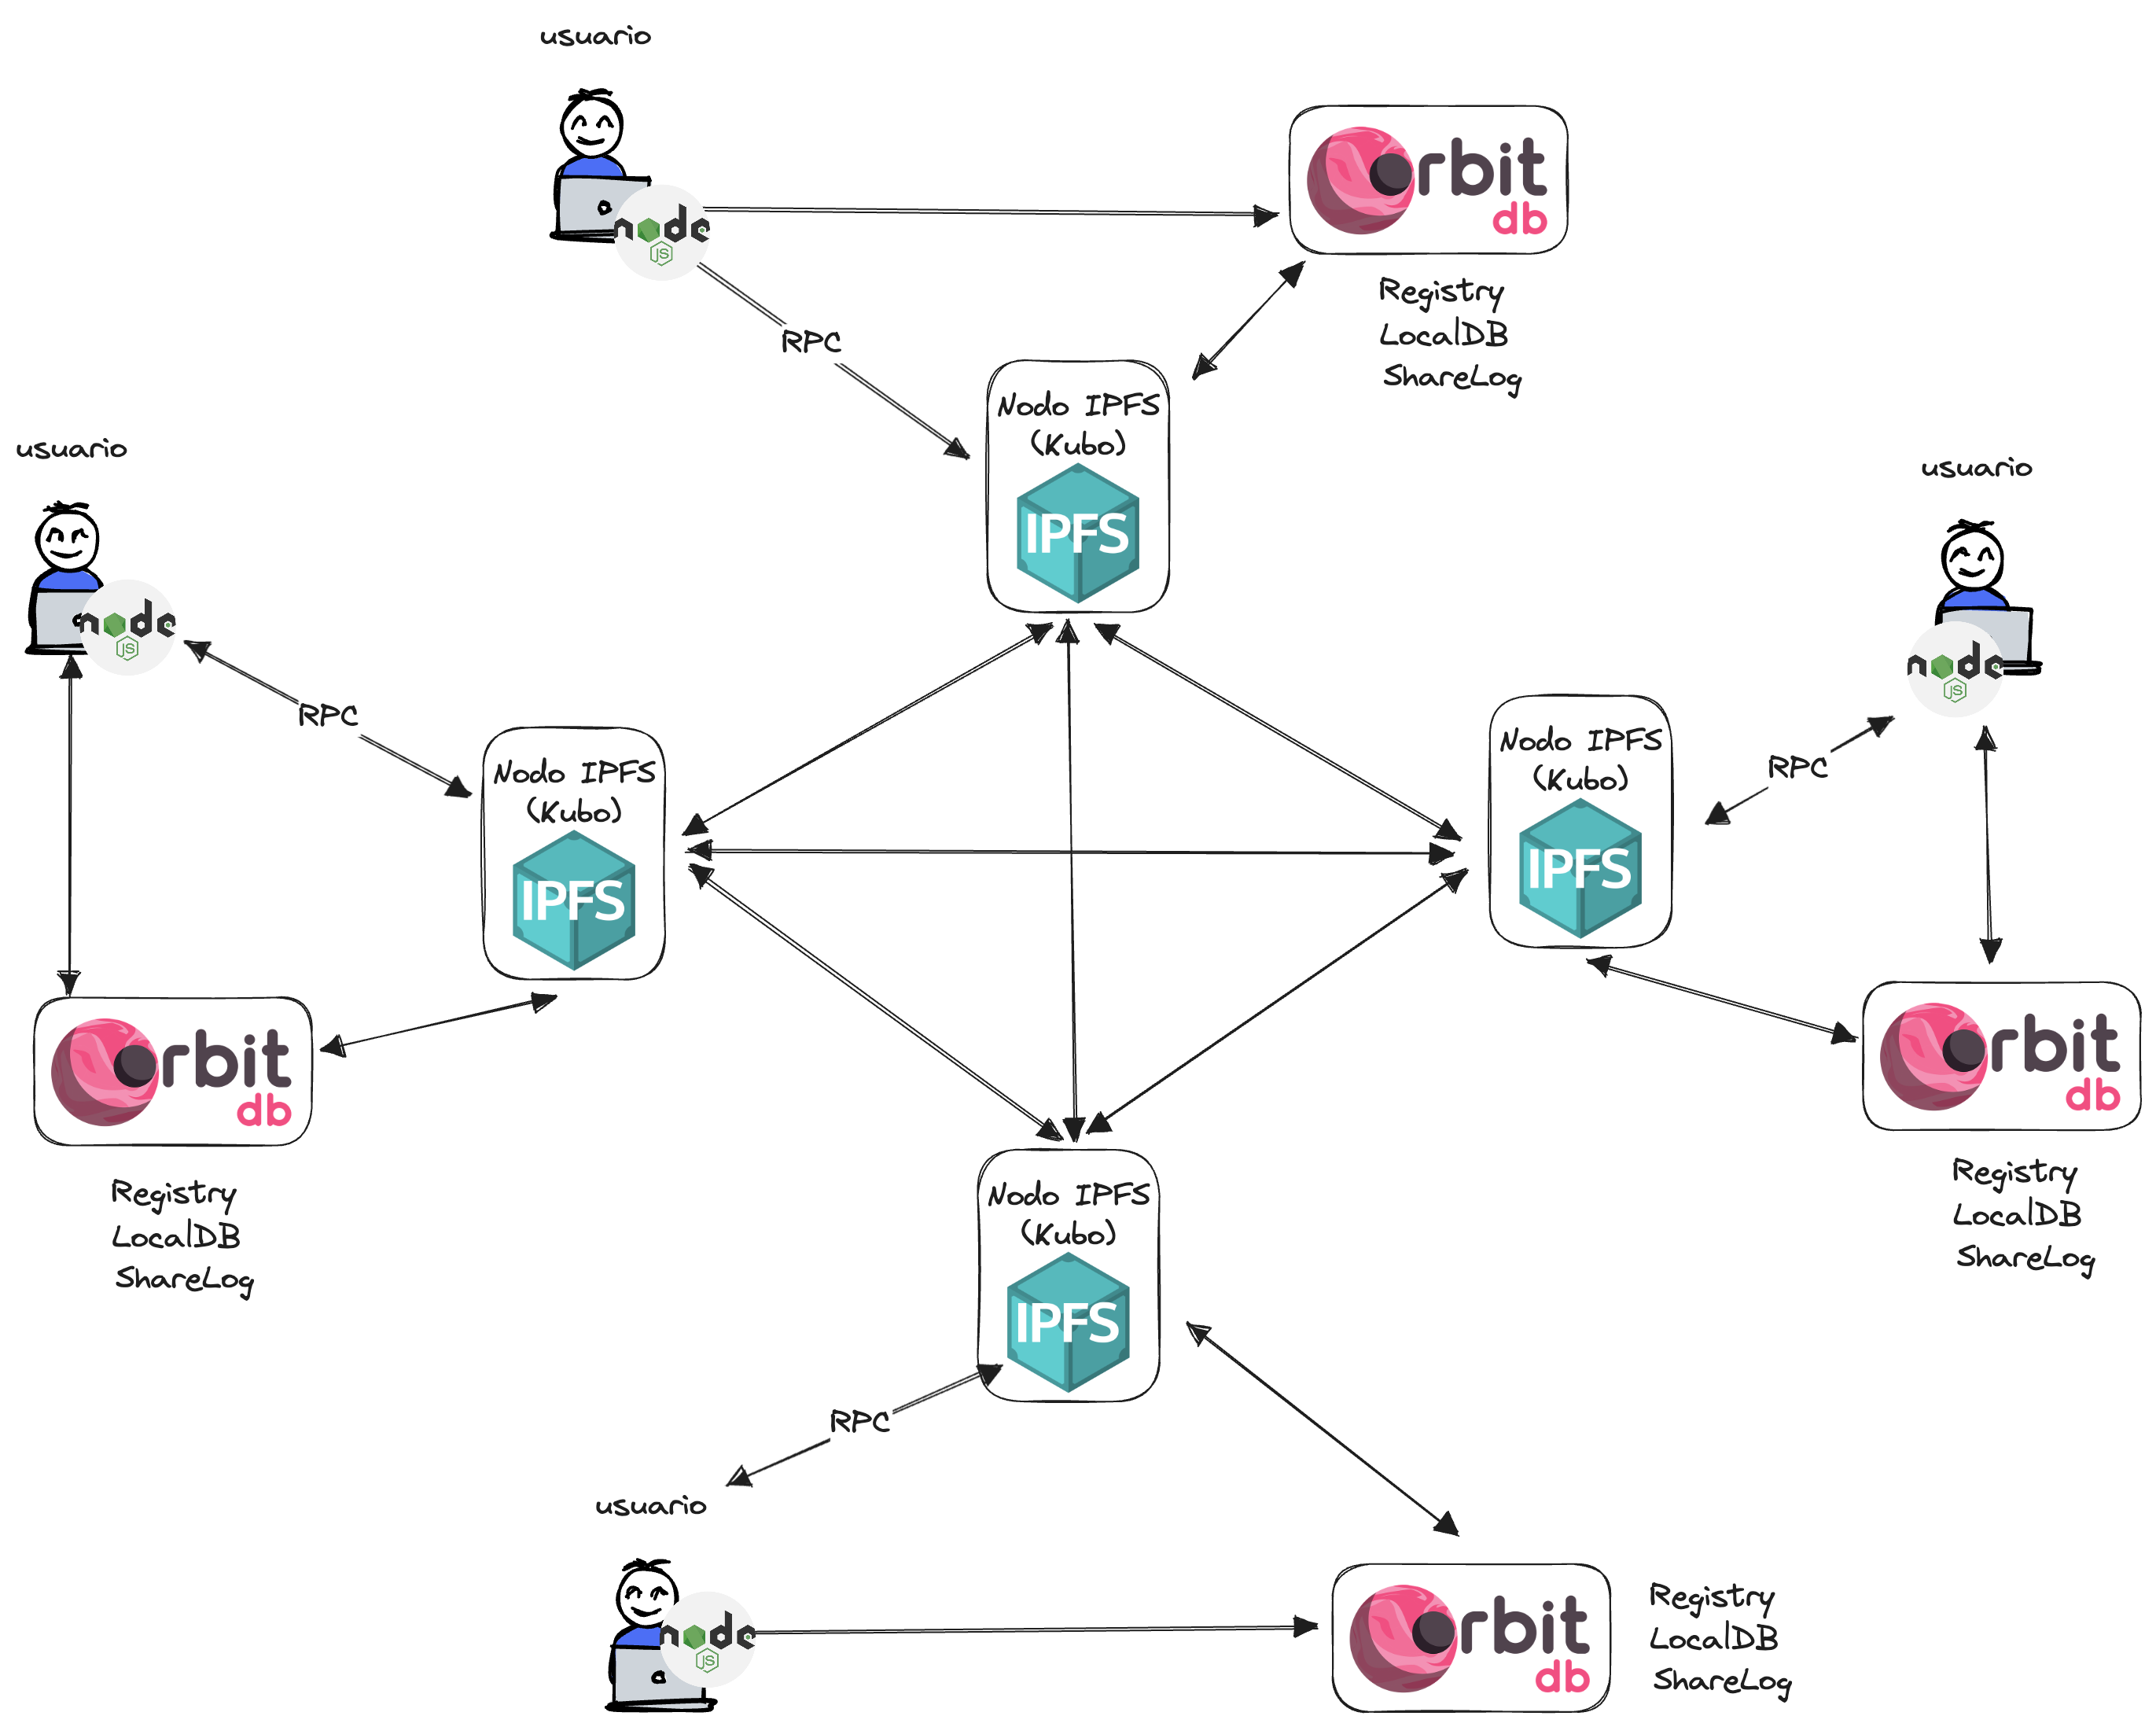
\includegraphics[width=\textwidth]{images/ipfshare-architecture.png}
  \caption{Arquitectura de IPFShare}
  \label{fig:ipfsharearch}
\end{figure}

En el sistema propuesto, cada usuario opera un nodo IPFS, que sirve como su punto de conexión a la red IPFS. Las interacciones entre el cliente y
este nodo IPFS se facilitan a través de una interfaz de programación de aplicaciones (API), que expone un conjunto de operaciones que puede realizar
el nodo \cite{KuboRPCAPI}. Esta comunicación se lleva a cabo mediante RPC, un protocolo que permite al cliente ejecutar procedimientos en el nodo IPFS como si estuvieran en el mismo sistema, lo que facilita la solicitud eficiente de servicios y operaciones.

El programa interactúa con la red IPFS mediante esta API a través del nodo IPFS local. IPFS sustituye al servicio de almacenamiento cloud
al ser un gran swarm de nodos que almacenan y comparten datos entre sí. IPFS en sí mismo no impone un límite teórico sobre la cantidad de datos que
pueden ser subidos a un nodo que se comporta correctamente. El límite práctico vendría determinado por factores como los recursos del sistema (espacio en
disco, ancho de banda de red, etc.), la configuración del nodo IPFS y cualquier restricción impuesta por la red o el proveedor de alojamiento. Proveedor
de alojamiento quiere decir otros nodos IPFS que compartan el mismo (o parte del) pinset que el nodo del usuario.

El servicio de procesamiento de ficheros se sustituye también por IPFS. El proceso de añadir cualquier dato a IPFS implica la subdivisión en chunks
para la generación del DAG y el uso de este en Bitswap, como ya se explicó en el apartado \ref{sect:modelo-de-datos}: '\nameref{sect:modelo-de-datos}'.

El servicio de autenticación se sustituye por un sistema de identificación descentralizado basado en DIDs que opera mediante
lo que se ha denominado como un \textit{Registry}. Un Registry es una base de datos distribuida que almacena información sobre los usuarios del sistema.
Esta base de datos distribuida es provista por OrbitDB, del cual se hablará más tarde en el apartado \ref{ssect:tecnologias}.

El concepto principal consiste
en que cada cliente tiene un instancia de OrbitDB que opera mediante IPFS. Esta instancia de OrbitDB mantiene constancia de una serie de bases de datos distribuidas que se sincronizan
con el resto de nodos, intercambiando los datos que se han modificado o añadido. De esta forma, se consigue una base de datos replicada y consistente entre todos los participantes del
sistema. OrbitDB ofrece diferentes tipos de bases de datos, como colecciones de documentos, claves-valor o registros de eventos. Para el caso del Registry, se utiliza una base de
datos de tipo clave-valor, donde la clave es el DID del usuario y el valor es un objeto JSON que contiene el peerID del usuario, su DID y un alias.
\begin{itemize}[noitemsep,after=\vspace{-0.4\baselineskip}]
  \item El DID es un identificador único que se genera a partir de la clave privada del usuario.
        Se utiliza como identidad de la instancia de OrbitDB para permitir verificar la autoría de las entradas en el registro.
  \item El alias es un nombre que el usuario puede elegir para identificarse en el sistema. Puede hacerse único o no, dependiendo de la política de acceso del Registry.
\end{itemize}

Un Registry debe incorporar un controlador de acceso que mantiene una serie de políticas de acceso respecto del mismo.
Estas políticas son:
\begin{itemize}[noitemsep,after=\vspace{-0.4\baselineskip}]
  \item Cualquier usuario puede crear una entrada en el registro.
  \item Un usuario solo puede tener una entrada en el registro.
  \item Solo el usuario que creó la entrada una puede modificarla.
  \item Solo el usuario que creó la entrada una puede eliminarla.
\end{itemize}


Cuando se crea una instancia de OrbitDB, el creador especifica un controlador de acceso (AC) para la base de datos.
Este controlador de acceso se almacena en el manifiesto de la base de datos (los metadatos de la base de datos)
y la dirección de este manifiesto se utiliza luego para cargar la base de datos. Entonces surge la pregunta, ¿no podría alguien simplemente intercambiar el controlador de acceso en su instancia local?
\\
La respuesta a esto es no, no pueden por las siguiente razones:
\begin{enumerate}[noitemsep,after=\vspace{-0.4\baselineskip}]
  \item El controlador de acceso y sus parámetros se almacenan en el manifiesto de la base de datos, y el hash de este manifiesto compone la dirección de la base de datos. Si alguien cambia el controlador de acceso, cambiarían el manifiesto, y por lo tanto la dirección de la base de datos. Esencialmente, estarían creando una base de datos completamente nueva, no alterando la original.
  \item Incluso si alguien crea una nueva base de datos con un controlador de acceso diferente, no pueden escribir en la base de datos original al no concordar las direcciones.
  \item Todas las actualizaciones a la base de datos (adiciones, modificaciones, etc.) son firmadas por las identidad del escritor. Si un usuario malintencionado intenta alterar los datos, las firmas no coincidirán, haciendo que los cambios sean invalidados por el resto de nodos que poseen la base datos.
  \item Al leer de la base de datos, el controlador de acceso valida si los datos (entradas) pueden ser añadidos a la base de datos local o no. Incluso si alguien cambiara el controlador de acceso localmente, no podrían alimentar datos alterados a otros porque los controladores de acceso de los demás validarían y rechazarían los cambios.
\end{enumerate}


El servicio de metadatos mediante colas de mensajes se sustituye por una base de datos distribuida de tipo
log, también provista por OrbitDB. Este componente se ha denominado en el sistema \textit{ShareLog}.
Un ShareLog es una base de datos distribuida que mantiene un registro de las acciones de compartición de los usuarios. Al realizar una compartición, el cliente añade una entrada al ShareLog, que contiene información sobre esta, que es distribuida entre todos los nodos del sistema. De esta forma, se consigue un registro de las comparticiones que se ha realizado en el sistema, que se puede consultar en cualquier momento. En este sistema cuando se habla
de notificaciones se refiere a entradas que llegan del ShareLog a los nodos clientes, que las procesan y muestran notificaciones al usuario, si es que están dirigidos a este.

El diagrama siguiente muestra como funciona la compartición en IPFShare:
\begin{figure}[H]
  \centering
  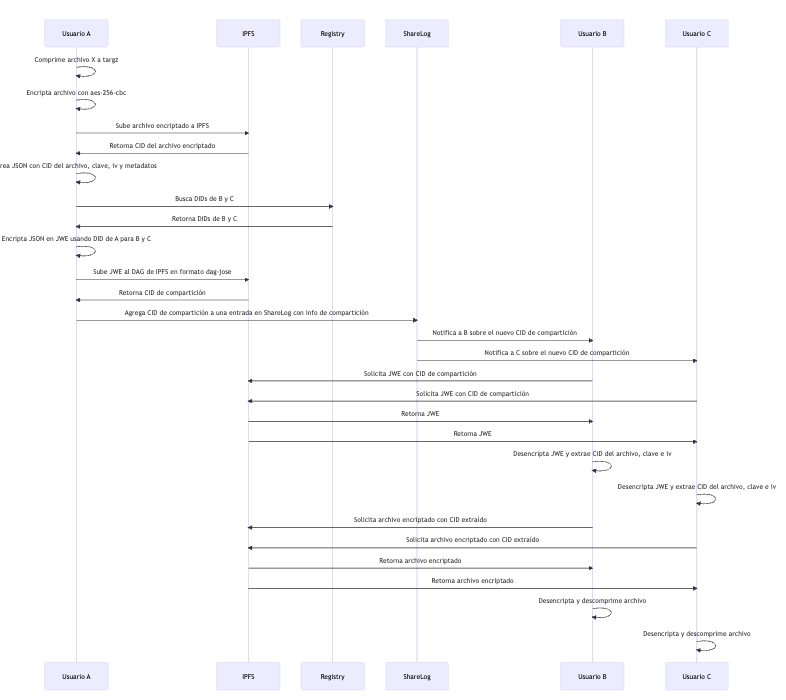
\includegraphics[width=\textwidth]{images/protocoloIpfshare.png}
  \caption{Protocolo de compartición implementado por IPFShare}
  \label{fig:ipfshareprotocol}
\end{figure}

En palabras este protocolo funciona de la siguiente forma:
\begin{itemize}[noitemsep,after=\vspace{-0.4\baselineskip}]
  \item Un archivo designado como ``X'' es comprimido en formato 'targz' por el usuario A.
  \item Posteriormente, el archivo comprimido es encriptado por el usuario A mediante el algoritmo aes-256-cbc.
  \item El archivo encriptado es subido al sistema Interplanetary File System (IPFS) por el usuario A. Como resultado de este proceso, el sistema IPFS devuelve un identificador de contenido (CID) correspondiente al archivo encriptado.
  \item El usuario A procede a la creación de un JSON que incluye el CID del archivo encriptado, la clave utilizada para la encriptación, el vector de inicialización (iv) y metadatos adicionales.
  \item El usuario A consulta el Registro (Registry) para obtener los Identificadores Descentralizados (DID) correspondientes a los usuarios B y C.
  \item Utilizando los DIDs obtenidos, el usuario A encripta el JSON previamente creado en un Token de Seguridad de JSON Encriptado (JWE). Esta encriptación se realiza de manera que únicamente los usuarios B y C pueden leer el contenido.
  \item El JWE es subido al Gráfico Acíclico Dirigido (DAG) de IPFS por el usuario A en formato dag-jose. En respuesta a esta operación, IPFS devuelve un CID correspondiente al JWE.
  \item Este CID, referido como el CID de compartición, es añadido por el usuario A a una entrada en el ShareLog con información detallada acerca de la compartición.
  \item ShareLog procede a notificar a los usuarios B y C sobre el nuevo CID de compartición.
  \item Los usuarios B y C solicitan a IPFS el JWE utilizando el CID de compartición. IPFS retorna el JWE a los usuarios.
  \item Posteriormente, los usuarios B y C desencriptan el JWE, y extraen de él el CID del archivo encriptado, la clave y el iv.
  \item Utilizando el CID extraído, los usuarios B y C solicitan a IPFS el archivo encriptado.
  \item Una vez obtenido, los usuarios B y C desencriptan y descomprimen el archivo utilizando la clave y el iv extraídos.
\end{itemize}

\section{Implementación}
Esta implementación se encuentra disponible en \href{https://github.com/nicocossiom/ipfshare}{Github} bajo la licencia MIT.
\subsection{Tecnologías usadas}\label{ssect:tecnologias}
\begin{itemize}[noitemsep,after=\vspace{-0.4\baselineskip}]
  \item \textbf{NodeJS:} Node.js es un entorno de ejecución (runtime) de JavaScript de código abierto, multiplataforma, que ejecuta código JavaScript fuera de un navegador web.
        NodeJS tiene una gran comunidad y dispone de una gran variedad de paquetes para uso dentro de su ecosistema. En este proyecto se usa NodeJS como runtime sobre el que se ejecuta la aplicación de línea de comandos IPFShare.
  \item \textbf{Typescript:} Typescript es un lenguaje de programación de código abierto desarrollado y mantenido por Microsoft. Es un superconjunto de JavaScript, que esencialmente añade tipos estáticos a Javascript. Se ha decidido usar este lenguaje en vez de JavaScript debido a que el tipado estático ayuda a detectar errores en tiempo de compilación, lo que facilita el desarrollo y reduce la cantidad de errores en tiempo de ejecución. Typescript realmente es transpilado a Javascriopt, esto permite usar
        paquetes de tipo ESM y CommonJS por igual sin tener que preocuparse por la compatibilidad entre los dos sistemas de módulos.
  \item \textbf{Paquetes/módulos de NodeJS}:
        \begin{itemize}[noitemsep]
          \item \texttt{archiver}: Proporciona funcionalidades para generar archivos comprimidos (por ejemplo, zip o tar) y trabajar con ellos.
          \item \texttt{chalk}: Herramienta para formatear y colorear el texto de la consola de Node.js.
          \item \texttt{cli-progress}: Permite crear barras de progreso en la interfaz de línea de comandos.
          \item \texttt{clipboardy}: Facilita el acceso al portapapeles del sistema para copiar y pegar.
          \item \texttt{commander}: Proporciona utilidades para escribir scripts de línea de comandos en Node.js.
          \item \texttt{did}: Biblioteca para trabajar con Identificadores Descentralizados (DIDs).
          \item \texttt{did-jwt}: Proporciona métodos para crear y verificar JWTs que usan DIDs.
          \item \texttt{did-resolver}: Ofrece funcionalidades para resolver DIDs a través de varios métodos.
          \item \texttt{dids}: Otra biblioteca para trabajar con DIDs, proporciona una API sencilla para crear y gestionar DIDs.
          \item \texttt{figlet}: Permite crear banners de texto ASCII.
          \item \texttt{fs-extra}: Proporciona métodos adicionales para trabajar con el sistema de archivos que no se incluyen en el módulo \texttt{fs} de Node.js.
          \item \texttt{go-ipfs}: Descarga el binario de IPFS, Kubo, en su útlima versión para su uso en cada plataforma.
          \item \texttt{inquirer}: Biblioteca para crear interfaces de usuario interactivas en la línea de comandos.
          \item \texttt{ipfsd-ctl}: Biblioteca para controlar un demonio IPFS desde Node.js.
          \item \texttt{key-did-provider-ed25519}: Proporciona un proveedor DID basado en el esquema de firma Ed25519.
          \item \texttt{key-did-resolver}: Ofrece métodos para la resolución de DIDs.
          \item \texttt{kubo-rpc-client}: Un cliente RPC para Kubo.
          \item \texttt{node-notifier}: Permite enviar notificaciones push nativas a cada plataforma dentro de Node.js.
          \item \texttt{ora}: Proporciona spinners elegantes para usar en la interfaz de línea de comandos.
          \item \texttt{orbit-db}: Base de datos peer-to-peer, construida sobre IPFS.
          \item \texttt{orbit-db-access-controllers}: Proporciona controladores de acceso para OrbitDB.
          \item \texttt{orbit-db-identity-provider}: Un proveedor de identidad para OrbitDB. Este paquete ha tenido que ser modificado para funcionar correctamente con DIDs como identidades debido a un error en su implementación. Disponible en \href{https://github.com/nicocossiom/orbit-db-identity-provider}{Github}.
          \item \texttt{orbit-db-keystore}: Almacén de claves para OrbitDB.
          \item \texttt{prompts}: Biblioteca para crear diálogos de usuario interactivos en la línea de comandos.
          \item \texttt{ps-list}: Ofrece una forma de enumerar todos los procesos en ejecución en el sistema.
          \item \texttt{tar}: Proporciona funcionalidades para trabajar con archivos tar.
          \item \texttt{winston}: Un logger flexible para Node.js.
        \end{itemize}

\end{itemize}

\subsubsection{Línea de comandos: CLI}\label{sssect:cli}
Se ha desarrollado una interfaz de línea de comandos (CLI) para facilitar el uso del sistema. Esta CLI se ha desarrollado usando CommanderJS.
Para crear una CLI en CommanderJS se sigue el siguiente patrón:
\begin{itemize}[noitemsep,after=\vspace{-0.4\baselineskip}]
  \item Se crea una instancia de Command.
  \item Se añaden comandos, opciones y argumentos a esta instancia usando una serie de métodos proporcionados.
  \item Se puede definir la acción a realizar al ejecutar cada comando.
  \item Se llama al método \texttt{parse} o \textit{parseAsync} para que CommanderJS procese los argumentos de la línea de comandos y ejecute las acciones correspondientes.
\end{itemize}

Por ejemplo:
\begin{minted}{typescript}
import { Argument, Command, Option, OptionValues } from "@commander-js/extra-typings"
const program = new Command()

program
    .version("0.0.1")
    .name("ipfshare")
    .addHelpText("before", `${chalk.yellow(logo)}`)
    .addHelpText("before", "An IPFS-based, encrypted file sharing CLI tool\n")
    .action(async () => {
        await notSetupPrompt()
        await daemonPromptIfNeeded() // checks if the daemon is running, if not it will prompt the user to start it
        program.help()
    })


    program.command("setup")
    .summary("Run initial setup")
    .description(`Runs the initial setup:
    - Creates IPFShare home folder. This is where all files/folders program related are located
    - Generate the IPFS repository and config
    - Generates encryption keys
    - Etc.`
    )
    .argument("[path]", "Path to IPFShare home folder") // Square brackets around the argument make it optional
    .action(async (path) => {
        if (path) {
            return await setupPrompt(path)
        }
        await setupPrompt()
    })
\end{minted}

Estos son los comandos implementados por IPFShare:

\begin{minted}{bash}
$ ipfshare --help
\end{minted}
\begin{verbatim}
,,
`7MMF'`7MM"""Mq.`7MM"""YMM  .M"""bgd `7MM
MM    MM   `MM. MM    `7 ,MI    "Y   MM
MM    MM   ,M9  MM   d   `MMb.       MMpMMMb.   ,6"Yb.  `7Mb,od8 .gP"Ya
MM    MMmmdM9   MM""MM     `YMMNq.   MM    MM  8)   MM    MM' "',M'   Yb
MM    MM        MM   Y   .     `MM   MM    MM   ,pm9MM    MM    8M""""""
MM    MM        MM       Mb     dM   MM    MM  8M   MM    MM    YM.    ,
.JMML..JMML.    .JMML.     P"Ybmmd"  .JMML  JMML.`Moo9^Yo..JMML.   `Mbmmd'
\end{verbatim}
\begin{minted}{text}
An IPFS-based, encrypted file sharing CLI tool

Usage: ipfshare [options] [command]

Options:
-V, --version                 output the version number
-h, --help                    display help for command

Commands:
setup [path]                  Run initial setup
daemon <action>               Start the Kubo (go-ipfs) daemon. This is a custom daemon for IPFShare. See daemon --help for more
info.
cat [cids...]                 Print the contents of a given CID
ls [cids...]                  List the contents of a given CID
share [path...]
download [options] [cids...]  Print the contents of a given CID
sharelog                      Interact with the global share log
shared                        List all files and folders shared with you
shares                        Interact with shares created by you
registry                      Access the IPFShare global registry. Change username or delete account.
info                          Provides information about the running ipfshare instance such as DID and peerID

\end{minted}


Cuando se ejecuta un comando la aplicación realiza todas las operaciones correspondientes dentro de lo que se ha denominado como \textit{Contexto}. El Contexto es un objeto que contiene todas las instancias de las clases que se necesitan para el correcto funcionamiento de la aplicación. Dado que existen interdependencias entre los componentes del Contexto este se tiene que iniciar en una secuencia específica.

\begin{minted}{typescript}
import { AppConfig } from "@app/common/appConfig"
import { UserRegistry } from "@app/registry"
import { IPFShareLog } from "@app/shareLog.js"
import { IPFSNodeManager } from "@ipfs/IPFSNodeManager.js"
import { DID } from "dids"
import type { Controller, ControllerType } from "ipfsd-ctl"
import { Socket } from "net"
import OrbitDB from "orbit-db"
import { Identity } from "orbit-db-identity-provider"

export interface AppContext {
  // fábrica de nodos IPFS preconfigurados
  manager: IPFSNodeManager | undefined
  orbitdb: OrbitDB | undefined // instancia de OrbitDB
  dbAddress: string | undefined // dirección de la base de datos
  identity: Identity | undefined // identidad de OrbitDB
  // DID de la identidad (es el mismo que identity pero en formato DID específico)
  did: DID | undefined 
  // el nodo IPFS o controlador
  ipfs: Controller<ControllerType> | undefined 
  // socket para comunicarse con el proceso daemon para el protocolo parada-espera
  daemonSocket: Socket | undefined 
  // el Registry global de IPFShare
  registry: UserRegistry | undefined
  // el ShareLog global de IPFShare
  shareLog: IPFShareLog | undefined
  // objeto con la configuración de la aplicación proviene de un archivo de la instalación
  appConfig: AppConfig | undefined // 
}
export async function withContext(fn: () => Promise<void>) {
  await initializeContext()
  await fn()
  await deInitializeContext()
}
\end{minted}
La función que se pasa como argumento a withContext se ejecuta dentro del contexto asegurando que este se ha inicializado correctamente, y que se desinicializa en el órden adecuado después de terminar la ejecución de la función.

Estas son las secuencias de inicialización y desinicialización del contexto:

\begin{minted}{typescript}
export async function initializeContext() {
  if (ctx.manager === undefined) {
// fábrica de nodos IPFS preconfigurados
    ctx.manager = await new IPFSNodeManager()
// crear un controlador (API RPC) que se conecta al daemon IPFS
    let ipfs : Controller<"go"> = await ctx.manager.createNode()
    ipfs = await ipfs.start().catch((err) => {
        logger.error(err)
        throw err
    })
    ctx.ipfs = ipfs
    ctx.daemonSocket = new net.Socket()
    ctx.daemonSocket.connect(3000, "localhost", () => {
        logger.info("Connected to the daemon process.") 
    })
    await sendMessageToOrbitDBService("pauseOrbitDB")
    ctx.orbitdb = await getOrbitDB()
    
    ctx.registry = new UserRegistry(ctx.ipfs.api, ctx.orbitdb)
    await ctx.registry.open()
    ctx.shareLog = new IPFShareLog(ctx.ipfs.api, ctx.orbitdb, "ipfs-sharelog")
    await ctx.shareLog.open()
    
    ctx.appConfig = await getAppConfigAndPromptIfUsernameInvalid()
  }
}
export async function deInitializeContext() {
  await ctx.registry?.store.close()
  await ctx.shareLog?.store.close()
  if (!ctx.orbitdb) throw new Error("OrbitDB instance undefined, not closed yet, should not happen")
  ctx.identity?.provider.keystore.close()
  await ctx.orbitdb?.disconnect()
  ctx.daemonSocket?.write("resumeOrbitDB")
  process.exit(0)
}
\end{minted}

\subsubsection{Protocolo parada-espera entre demonio y CLI}

Como se puede observar dentro del Contexto se implementa parte del protocolo parada espera
que comunica con el proceso demonio que se ejecuta en segundo plano. Este protocolo se ha implementado
para poder usar dos instancias de OrbitDB bajo el mismo directorio de datos.

Esto es necesario ya que el demonio siempre está en ejecución, con su instancia de OrbitDB mantieniendo las
bases de datos actualizadas y sincronizadas con el resto de nodos. Cuando se ejecuta la CLI, esta instancia de OrbitDB se pausa para que la CLI pueda
'\textit{robar}' la instancia al demonio (la vuelve a crear). Cuando se termina la ejecución de la CLI, se reanuda la instancia de OrbitDB del demonio para que este pueda seguir funcionando, retransmitiendo las operaciones que haya realizado la CLI.

\begin{figure}[H]
  \centering
  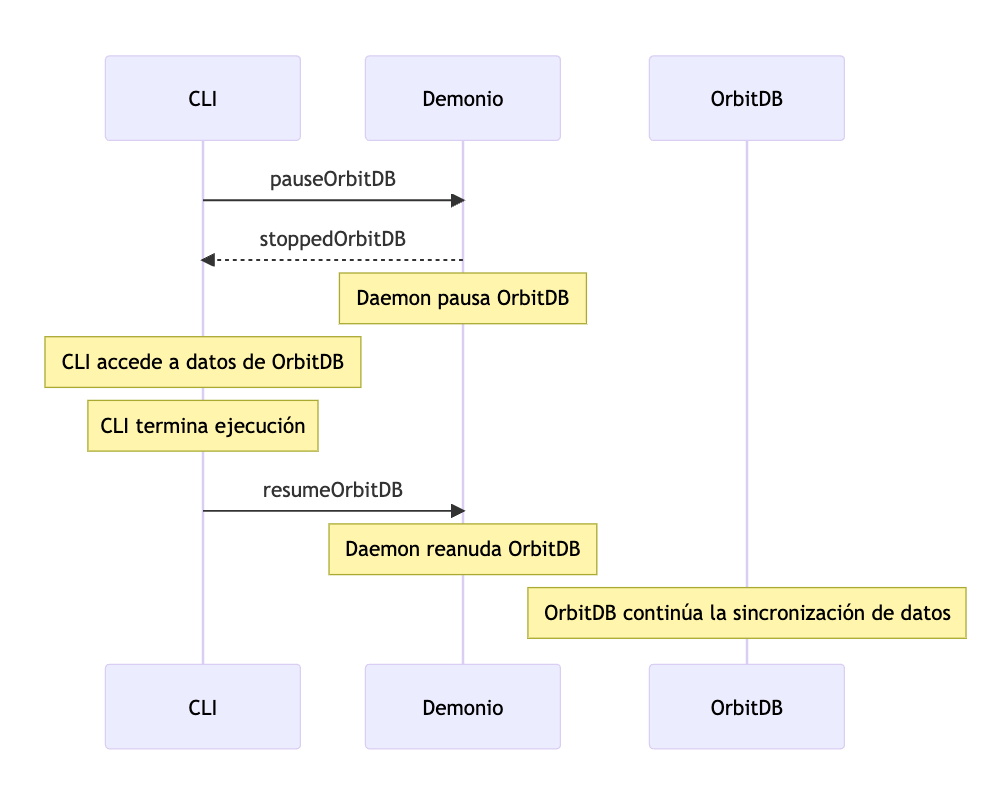
\includegraphics[width=\textwidth]{images/parada-espera-orbitdb.png}
  \caption{Diagrama de secuencia del protocolo parada-espera implementado}
  \label{fig:parada-espera}
\end{figure}

La comunicación se realiza mediante un socket TCP en el puerto 3000 (se podría configurar en cualquier otro puerto). El protocolo es muy sencillo: el cliente envía un mensaje al servidor, el servidor lo procesa y responde con otro mensaje de confirmación. El cliente espera a recibir este mensaje para continuar con la ejecución. Cuando termina manda otro mensaje al servidor para que este retome donde lo había dejado.

\begin{minted}{typescript}
// esta es la función que se encarga de enviar comunicarse con proceso demonio
function sendMessageToOrbitDBService(message: string): Promise<string> {
  return new Promise((resolve, reject) => {
      if (ctx.daemonSocket === undefined ) throw new Error("Daemon socket is undefined")
      ctx.daemonSocket.once("data", data => {
          // Handle any response or acknowledgment from the daemon process
          const response = data.toString()
          logger.debug(`Received response for message ${message}:`, response)
          resolve(response)
      })

      ctx.daemonSocket.write(message, error => {
          if (error) {
              console.error("Error sending message:", error.message)
              reject(error)
          }
          logger.debug(`Sent message ${message}`)
      })
  })
}
// este servicio es creado por el proceso demonio y se encarga de procesar los mensajes que recibe de la CLI
private static createOrbitDBService() {
const server = net.createServer(socket => {
  socket.on("data", data => {
    const message = data.toString()

    if (message === "pauseOrbitDB") {
        (async () => {
            logger.info("Pausing OrbitDB")
            if (!ctx.orbitdb) throw new Error("OrbitDB is not initialized")
            await ctx.orbitdb.disconnect()
            if (!process.env.IPFSHARE_HOME) throw new Error("IPFShare home is not set")
            ctx.identity?.provider.keystore.close()
            socket.write("OrbitDB paused")
        })()
    }
    else if (message === "resumeOrbitDB") {
        (async () => {
            logger.info("Resuming OrbitDB")
            if (!ctx.ipfs) throw new Error("IPFS is not initialized")
            ctx.orbitdb = await getOrbitDB(true)
            await ctx.identity?.provider.keystore.open()
            ctx.registry = new UserRegistry(ctx.ipfs.api, ctx.orbitdb)
            await ctx.registry.open()
            logger.info("Replicating registry")
            await ctx.registry.replicate()
            ctx.shareLog = new IPFShareLog(ctx.ipfs.api, ctx.orbitdb, "ipfs-sharelog")
            await ctx.shareLog.open()
            await ctx.shareLog.onNewShare()
        })()
    }
  })
  socket.on("error", err => {
      logger.error("Error in OrbitDB service", err)
      throw err
  })
})

return server
}
\end{minted}

\subsubsection{Proceso demonio}


\begin{minted}{typescript}

public async startDaemon(): Promise<void> {
  const service = IPFSNodeManager.createOrbitDBService()
  service.listen(3000, "localhost", () => { 
      logger.info("OrbitDB service listening on port 3000")
  })
  let daemon = await this.createNode()
  daemon = await daemon.start()
      .catch((err) => { 
          logger.error("Error launching daemon", err) 
          process.exit(1)
      })
  daemon.subprocess?.stdout?.pipe(process.stdout)
  daemon.subprocess?.stderr?.pipe(process.stderr)
  daemon.subprocess?.setMaxListeners(Infinity)
  logger.debug(`IPFS Daemon started with pid ${daemon.subprocess?.pid}`)
  ctx.ipfs = daemon
  ctx.orbitdb = await getOrbitDB(true)
  ctx.registry = new UserRegistry(ctx.ipfs.api, ctx.orbitdb)
  logger.info("Replicating registry")
  await ctx.registry.open()
  await ctx.registry.replicate()
  ctx.shareLog = new IPFShareLog(ctx.ipfs.api, ctx.orbitdb, "ipfs-sharelog")
  await ctx.shareLog.open()
  await ctx.shareLog.onNewShare()
  ctx.appConfig = await getAppConfigAndPromptIfUsernameInvalid(true)
  process.on("SIGINT", () => {
      (async () => {
          logger.info("Killing daemon")
          await daemon.stop()
          fs.rmSync(path.join(IPFSNodeManager.getRepoPath(), "api"), {force:true})
          await ctx.orbitdb?.disconnect()
          process.exit(0)
      })()
  })

  process.on("beforeExit", () => {
      (async () => {
          logger.info("Daemon exiting")
          await daemon.stop()
          fs.rmSync(path.join(IPFSNodeManager.getRepoPath(), "api"), {force:true})
          process.exit(0)
      })()
  })
}
public static async stopDaemon(): Promise<void> {
  // get the pid of the daemon
  const pid = await psList().then((list) => {
      const daemon = list.find((someProcess) => someProcess.name.includes("node_modules/go-ipfs/bin/ipfs"))
      if (daemon === undefined) {
          return undefined 
      }
      return daemon.pid
  })
  if (pid === undefined) {
      console.error("Could not find daemon")
      return
  }
  // kill the daemon
  process.kill(pid)
}  
\end{minted}

La invocaicón de este proceso se realiza mediante el comando \texttt{ipfshare daemon <action>}. Las acciones disponibles son:
\begin{itemize}[noitemsep,after=\vspace{-0.4\baselineskip}]
  \item \texttt{start}: Inicia el proceso demonio.
  \item \texttt{stop}: Detiene el proceso demonio.
\end{itemize}



\subsubsection{Registry}

El Registry se ha representado en una clase abstracta que define la interfaz que debe implementar cualquier Registry que se quiera usar en el sistema. Esta clase abstracta se ha definido de la siguiente forma:
\begin{minted}{typescript}
import { IPFS } from "kubo-rpc-client/dist/src/types"
import OrbitDB from "orbit-db"
import AccessController from "orbit-db-access-controllers/interface"
import DocumentStore from "orbit-db-docstore"
import { IdentityProvider } from "orbit-db-identity-provider"
// S es el tipo de Store de Orbit que se desee usar (DocumentStore, KeyValueStore, etc.)
// DocType es el tipo de documento que se va a almacenar en el Store
// AccessController es un controlador de acceso que debe implementar las políticas de acceso al Registry ya explicadas
export abstract class Registry<S, DocType> {
    abstract accessController: AccessController
    abstract store: S
    abstract open(): Promise<void> 
    abstract create(): Promise<void>
    abstract replicate(): Promise<void>
    abstract close(): Promise<void>
    abstract addUser(user: DocType): Promise<void>
    abstract getUser(entryId: string): Promise<DocType | undefined>
    abstract updateUser(entryId: string, updates: Partial<DocType>): Promise<void>
    abstract searchUsers(queryFn: (entry: DocType) => boolean): Promise<DocType[]>
    abstract deleteUser(entryId: string): Promise<void>
}
\end{minted}
Se ha implemntado un controlador de acceso básico \\'\texttt{IPFShareRegistryAccessController}' que implementa las políticas de acceso al
Registry:

\begin{minted}{typescript}
export class IPFShareRegistryAccessController extends AccessController{
  _orbitdb: OrbitDB
  _registry: Registry<any, any>

  constructor(orbitdb: OrbitDB, registry: Registry<any, any>) {
    super()
    this._orbitdb = orbitdb
    this._registry = registry
  }
  // este es el método al que llama OrbitDB para comprobar si se puede añadir una entrada al Registry
  async canAppend(entry: LogEntry<any>, identityProvider: IdentityProvider): Promise<boolean> {
    const userId = await entry.identity.id
    if (!userId) {
        throw new Error("identity is not set")
    }
    logger.debug(`Registry: ${userId} is trying to append`)
    const existingUser = await this._registry.getUser(userId)

    // Only allow appending to the log if the user does not exist or the user is the owner
    if (!existingUser || existingUser.orbitdbIdentity === entry.identity.id) {
        logger.debug(`Registry: ${userId} authorized to append`)
        // Allow access if identity verifies
        return true
    }
    logger.debug(`Registry: ${userId} NOT authorized to append`)
    return false
  }

  static get type(): string {
      return "ipfshare-registry"
  }

  save(): Promise<any> {
    return Promise.resolve({})
  }

  get address(): string {
    return this._registry.store.address.toString()
  }

  static async create(orbitdb: OrbitDB, options:{registry: Registry<any, any>}): Promise<AccessController> {
    // options must contain the registry to be used for access control
    return new IPFShareRegistryAccessController(orbitdb, options.registry) 
  }
}
\end{minted}

IPFShare implementa un Registry propio que se ha denominado '\texttt{UserRegistry}'. Las entradas en este Registry
son de tipo \texttt{RegistryEntry}:
\begin{minted}{typescript}
export interface RegistryEntry {
  peerId: string
  orbitdbIdentity: string // DID
  username: string // alias
}
\end{minted}
\begin{minted}{typescript}
export class UserRegistry implements Registry<DocumentStore<RegistryEntry>, RegistryEntry> {
store: DocumentStore<RegistryEntry>
orbitdb: OrbitDB
ipfs: IPFS
accessController: IPFShareRegistryAccessController

constructor(ipfs: IPFS, orbitdb: OrbitDB) {
  this.ipfs = ipfs
  this.orbitdb = orbitdb
  this.store = {} as DocumentStore<RegistryEntry>
  this.accessController = new IPFShareRegistryAccessController(orbitdb, this)
}

async open(): Promise<void> {
  try {
    this.store = await this.orbitdb.docstore<RegistryEntry>(
        "ipfshare-registry",
        {
            accessController: {
                type: IPFShareRegistryAccessController.type,
                registry: this,                  
            },
            // esta es la clave por la que se indexan los documentos del Registry
            indexBy: "orbitdbIdentity", 
        }
    )
    await this.store.load()
  } catch (e) {
    // si falla open es porque la base de datos no existe, hay que crearla
    await this.create()
  }
}

async close(): Promise<void>{
    await this.store.close()
}

async create(): Promise<void> {
  try {
    this.store = 
      await this.orbitdb.docstore("ipfshare-registry", 
        {
          accessController: {
                type: IPFShareRegistryAccessController.type,
                registry: this,
            },
            create: true, // se añade esta opción para que se cree la base de datos si no existe
            indexBy: "orbitdbIdentity",

        }
      )
  }catch (e) {
    logger.error(e)
  }
}

// este método es llamado por el demonio para replicar el Registry
async replicate(): Promise<void> {
  await this.store.load()
  this.store.events.on("replicated", (address) => {
      logger.info(`Registry replicated ${address} `)
  })
  this.store.events.on("replicate", (address) => {
      logger.info(`Registry replicate ${address} `)
  })
  // cuando se conecta un nuevo nodo al sistema recargamos el Registry
  this.store.events.on("peer", (peer) => {
      (async () => {
          await this.store.load()
      })()
      logger.info(`Registry peer connected ${peer}`)
  })
  this.store.events.on("replicate.progress", (address, hash, entry, progress, have) => {
      logger.info(`Registry replication progress ${address}, ${hash}, ${entry}, ${progress}, ${have}`)
  })
  this.store.events.on("peer.exchanged", (peer, address, heads) => {
      logger.info(`Registry\n\tpeer ${peer} exchanged, ${heads.toString()}`)
  } )
}

async addUser(user: RegistryEntry): Promise<void> {
  if (!user.username) throw new Error("Username is not set")
  await this.store.put(user)
}

async getUser(entryId: string): Promise<RegistryEntry | undefined> {
  const matchingUsers = this.store.get(entryId)
  if (matchingUsers.length === 0) return undefined
  if (matchingUsers.length > 1) throw new Error("Multiple users with the same username")
  return matchingUsers[0]
}

async updateUser(entryId: string, updates: Partial<RegistryEntry>): Promise<void> {
  const oldEntry = await this.getUser(entryId)
  if (!oldEntry) throw new Error("User not found")
  const newEntry = {
      ...oldEntry,
      ...updates
  } as RegistryEntry
  this.store.put(newEntry)
}

async deleteUser(entryId: string): Promise<void> {
    const user = await this.getUser(entryId)
    if (!user) {
        throw new Error("User not found")
    }
    await this.store.del(entryId)
}

async searchUsers(mapper: (entry: RegistryEntry) => boolean): Promise<RegistryEntry[]> {
    const allUsers = this.store.query(mapper)
    return allUsers
}}
\end{minted}

\subsubsection{Compartición de un archivo}
En la CLI se ha implementado un comando para compartir archivos y carpetas. Este comando se ha implementado de la siguiente forma:
\begin{minted}{typescript}
program.command("share")
  .argument("[path...]", "Path to file or folder to upload")
  .action(async (paths) => {
      if (!paths || paths.length === 0) {
          program.help()
      }
      await withContext(async () => {
          if (!ctx.did) throw new Error("DID not initialized")
          const { encryptedStream, iv, key } = await createEncryptedTarFromPaths(paths)
          const res = await uploadToIpfs(encryptedStream)
          console.log(`Uploaded to IPFS with CID: ${res.cid.toString()}, size: ${res.size}`)
          const recipients: string[] = await interactiveRegistryPrompt("Select recipients")
          recipients.push(ctx.appConfig!.user.orbitdbIdentity)
          console.log(`Recipient DIDs ${recipients}`)
          const share: Share = {
              contentCID: res.cid, 
              iv: iv.toString("base64"), 
              key: key.toString("base64"), 
              recipientDIDs: recipients
          }
          const msg = await messagePrompt()
          const recipientNames= getRecipientNames(share.recipientDIDs)
          const shareCID = await addEncryptedObject(share)
          const shareHash = await ctx.shareLog?.addShare(
              {
                  message: msg,
                  recipients: recipients,
                  shareCID: shareCID,
                  senderName: ctx.appConfig!.user.username,
                  recipientNames: recipientNames, 
                  senderId: ctx.appConfig!.user.orbitdbIdentity
              }
          ) 
          console.log(`Added share to ShareLog with hash: ${shareHash}`)
          console.log(`Content CID: ${res.cid.toString()}`)
          console.log(`Share CID: ${shareCID.toString()}`)
      })
  })
\end{minted}

'\textit{'interactiveRegistryPrompt}' es un método que muestra un diálogo interactivo para seleccionar los usuarios con los que se quiere compartir el archivo. Este diálogo se ha implementado con la biblioteca \texttt{prompts}.

\begin{minted}{typescript}
const interactiveRegistryPrompt:  (promptMessage: string)  => Promise<string[]> = async (promptMessage) => {
  const users =  (await ctx.registry?.searchUsers(() => true))
  if (!users) throw new Error("No users found")
  const choices = users.filter(user => ctx.appConfig?.user.peerId !== user.peerId)
      .map((user) => {
          const res: prompts.Choice = {
              title: `${user.username} - ${user.orbitdbIdentity} - peerId: ${user.peerId}`,
              value: user.orbitdbIdentity,
          }
          return res
      })
  // using prompts package with autocompleteMultiselect
  const response = await prompts.prompt({
      type: "autocompleteMultiselect",
      name: "recipients",
      message: promptMessage,
      choices: choices,
      min: 0,
      max: users.length,
      hint: "- Space to de/select. Return to submit"
  })

  if (response.recipients) {
      return response.recipients
  } else {
      throw new Error("No recipients selected")
  }
}
\end{minted}

Esto es solo un ejemplo de las posibilidades que ofrece el Registry. Los datos y metadatos, además de la complejidad dependen de la la implementación
de este. El concepto de Registry es muy flexible y se puede adaptar a cualquier necesidad (dentro de unas limitaciones).

